\documentclass{ltjsarticle}
\usepackage{luatexja}
\usepackage{luatexja-fontspec}
\usepackage[no-math,deluxe,expert,ipaex]{luatexja-preset}
% 数式関係
\usepackage{amsmath, amssymb}
\usepackage{mathtools}
\usepackage{bm}
\usepackage[italicdiff]{physics}
\usepackage{empheq}
% ローマ数字
\usepackage{romannum}
% 強制配置
\usepackage{here}
% table関係
\usepackage{booktabs, tabularray, longtable}
% pdf読み込み
\usepackage{pdfpages}
% 単位
\usepackage{siunitx}
% 箇条書き
\usepackage[inline]{enumitem}
% tikz
\usepackage{tikz}
% 回路図
\usepackage{circuitikz}
% ブロック線図
\usepackage{blox}
% subcaption関係
\usepackage[hang,small,bf]{caption}
\usepackage[subrefformat=parens]{subcaption}
\captionsetup{compatibility=false}
% cleveref
\usepackage{cleveref}
\usepackage{etoolbox}
\cslet{blx@noerroretextools}\empty
% \usepackage{autonum}

\crefname{defn}{定義}{定義}%
\crefname{thm}{定理}{定理}%
\crefname{lem}{補題}{補題}%
\crefname{coro}{系}{系}%
\crefname{prop}{命題}{命題}%
\crefname{ex}{例}{例}%
\crefname{rem}{注意}{注意}%

\newcommand{\crefrangeconjunction}{{〜}}%
\newcommand{\crefrangepreconjunction}{}%
\newcommand{\crefrangepostconjunction}{}%
\newcommand{\crefpairconjunction}{, }%
\newcommand{\crefmiddleconjunction}{, }%
\newcommand{\creflastconjunction}{, }%
\newcommand{\crefpairgroupconjunction}{, }%
\newcommand{\crefmiddlegroupconjunction}{, }%
\newcommand{\creflastgroupconjunction}{, }%

\crefname{equation}{式}{式}%
\crefname{figure}{図}{図}%
\crefname{subfigure}{図}{図}%
\crefname{table}{表}{表}%
\crefname{subtable}{表}{表}%

\crefname{appendix}{付録}{付録}%
\crefname{subappendix}{付録}{付録}%
\crefname{subsubappendix}{付録}{付録}%
\crefname{subsubsubappendix}{付録}{付録}%

\crefformat{page}{#2#1#3{ページ}}%
\crefrangeformat{page}{#3#1#4{〜}#5#2#6{ページ}}%
\crefmultiformat{page}{#2#1#3{ページ}}%
  {, #2#1#3{ページ}}{, #2#1#3}{, #2#1#3{ページ}}%
\crefformat{section}{#2#1#3{節}}%
\crefrangeformat{section}{#3#1#4{〜}#5#2#6{節}}%
\crefmultiformat{section}{#2#1#3{節}}%
  {, #2#1#3{節}}{, #2#1#3}{, #2#1#3{節}}%
\crefformat{subsection}{#2#1#3{節}}%
\crefrangeformat{subsection}{#3#1#4{〜}#5#2#6{節}}%
\crefmultiformat{subsection}{#2#1#3{節}}%
  {, #2#1#3{節}}{, #2#1#3}{, #2#1#3{節}}%
\crefformat{subsubsection}{#2#1#3{節}}%
\crefrangeformat{subsubsection}{#3#1#4{〜}#5#2#6{節}}%
\crefmultiformat{subsubsection}{#2#1#3{節}}%
  {, #2#1#3{節}}{, #2#1#3}{, #2#1#3{節}}%

\crefformat{part}{{第}#2#1#3{部}}%
\crefformat{chapter}{{第}#2#1#3{章}}%

% ソースコード貼り付け
\usepackage{listings, jvlisting}
\lstset{
%枠外に行った時の自動改行
breaklines = true,
%自動改行後のインデント量(デフォルトでは20[pt])
breakindent = 10pt,
%標準の書体
basicstyle = \ttfamily\scriptsize,
%コメントの書体
commentstyle = {\itshape \color[cmyk]{1,0.4,1,0}},
%関数名等の色の設定
classoffset = 0,
%キーワード(int, ifなど)の書体
keywordstyle = {\bfseries \color[cmyk]{0,1,0,0}},
%表示する文字の書体
stringstyle = {\ttfamily \color[rgb]{0,0,1}},
%枠 tは上に線を記載, Tは上に二重線を記載
%他オプション:leftline,topline,bottomline,lines,single,shadowbox
frame = tb,
%frameまでの間隔(行番号とプログラムの間)
framesep = 5pt,
%行番号の位置
numbers = left,
%行番号の間隔
stepnumber = 1,
%行番号の書体
numberstyle = \tiny,
%タブの大きさ
tabsize = 4,
%キャプションの場所(tbならば上下両方に記載)
captionpos = t
}

% 参考文献
\usepackage[
  backend=biber,
  sorting=none
]{biblatex}

\begin{document}
\setcounter{page}{1}
\pagenumbering{arabic}

\section{目的}
現在,産業用ロボットは,その精密な作業や人間が入ることのできない過酷な環境下での活躍,そして効率化など,工業の分野においてなくてはならない存在となっている.その中でも,ロボットアームは,見た目の動作が直感的であり,エンドエフェクタを取り替えることによりさまざまな作業ができることから,自動車産業をはじめとして幅広く使われている.

本実験では,6自由度のロボットアームを使ってシミュレーションと実際の操作を行い,ロボット工学の基礎である
\begin{enumerate*}
	\item DH法による座標系のとりかた
	\item 同次変換行列
	\item 順運動学
	\item 逆運動学
\end{enumerate*}
について学ぶ.

\section{実験装置と開発環境}
本実験では,6自由度の小型ロボットアーム,"myCobot 280 Pi"を用いる.これは,Raspberry Piが組み込まれているため,OSを直接操作やssh接続してOSを遠隔操作するなどしてロボットを動かすことができる.

今回は自分のPCからssh接続して,OSを遠隔操作することによりロボットを操作した.なお,シミュレーションの実行環境を\cref{tab:実行環境}に示す.
\begin{table}[H]
	\centering
	\caption{実行環境}
	\label{tab:実行環境}
	\begin{tblr}{
		cells = {halign = l},
		hline{1,Z} = {0.08em}
	}
		OS & Ubutnu 24.04 \\
		Pythonの実行環境 & Python 3.12.3 (venv)
	\end{tblr}
\end{table}

\section{実験}
\subsection{DH法によりリンク間の座標$\Sigma_i$を定義}
\cref{fig:ロボットアームのモデルと座標系-直立状態}に,直立状態のロボットアームのモデルを示す.まず,DH法によりリンク間の座標を定義していく.\cref{fig:ロボットアームのモデルと座標系-直立状態}より,関節はすべて回転関節であるから,$z_i$はすべて回転に対して右ねじの向きにとる.次に,隣接する関節どうしの$z$軸の関係について,交錯する組と平行の組が\cref{tab:隣接する関節どうしのz軸の関係}のようにわけられる.
\begin{table}[H]
	\centering
	\caption{隣接する関節どうしの$z$軸の関係}
	\label{tab:隣接する関節どうしのz軸の関係}
	\begin{tblr}{
		cells = {halign = l},
		hline{1,Z} = {0.08em}
	}
		交錯 & $(z_0, z_1), (z_3, z_4), (z_4, z_5)$ \\
		平行 & $(z_1, z_2), (z_2, z_3), (z_5, z_6)$
	\end{tblr}
\end{table}

\cref{tab:隣接する関節どうしのz軸の関係}の関係に気をつけて座標$\Sigma_i$を定義していくと,\cref{fig:ロボットアームのモデルと座標系-DH法により座標系を定義}の形で座標系が定義できる.
\begin{figure}[H]
	\centering
	\begin{tabular}{cc}
		\begin{minipage}[c]{0.48\linewidth}
			\centering
			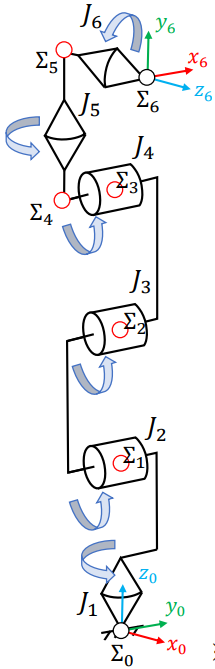
\includegraphics[width = 0.7\linewidth]{../figures/robot_arm_0.png}
			\subcaption{直立状態}
			\label{fig:ロボットアームのモデルと座標系-直立状態}
		\end{minipage}
		&
		\begin{minipage}[c]{0.48\linewidth}
			\centering
			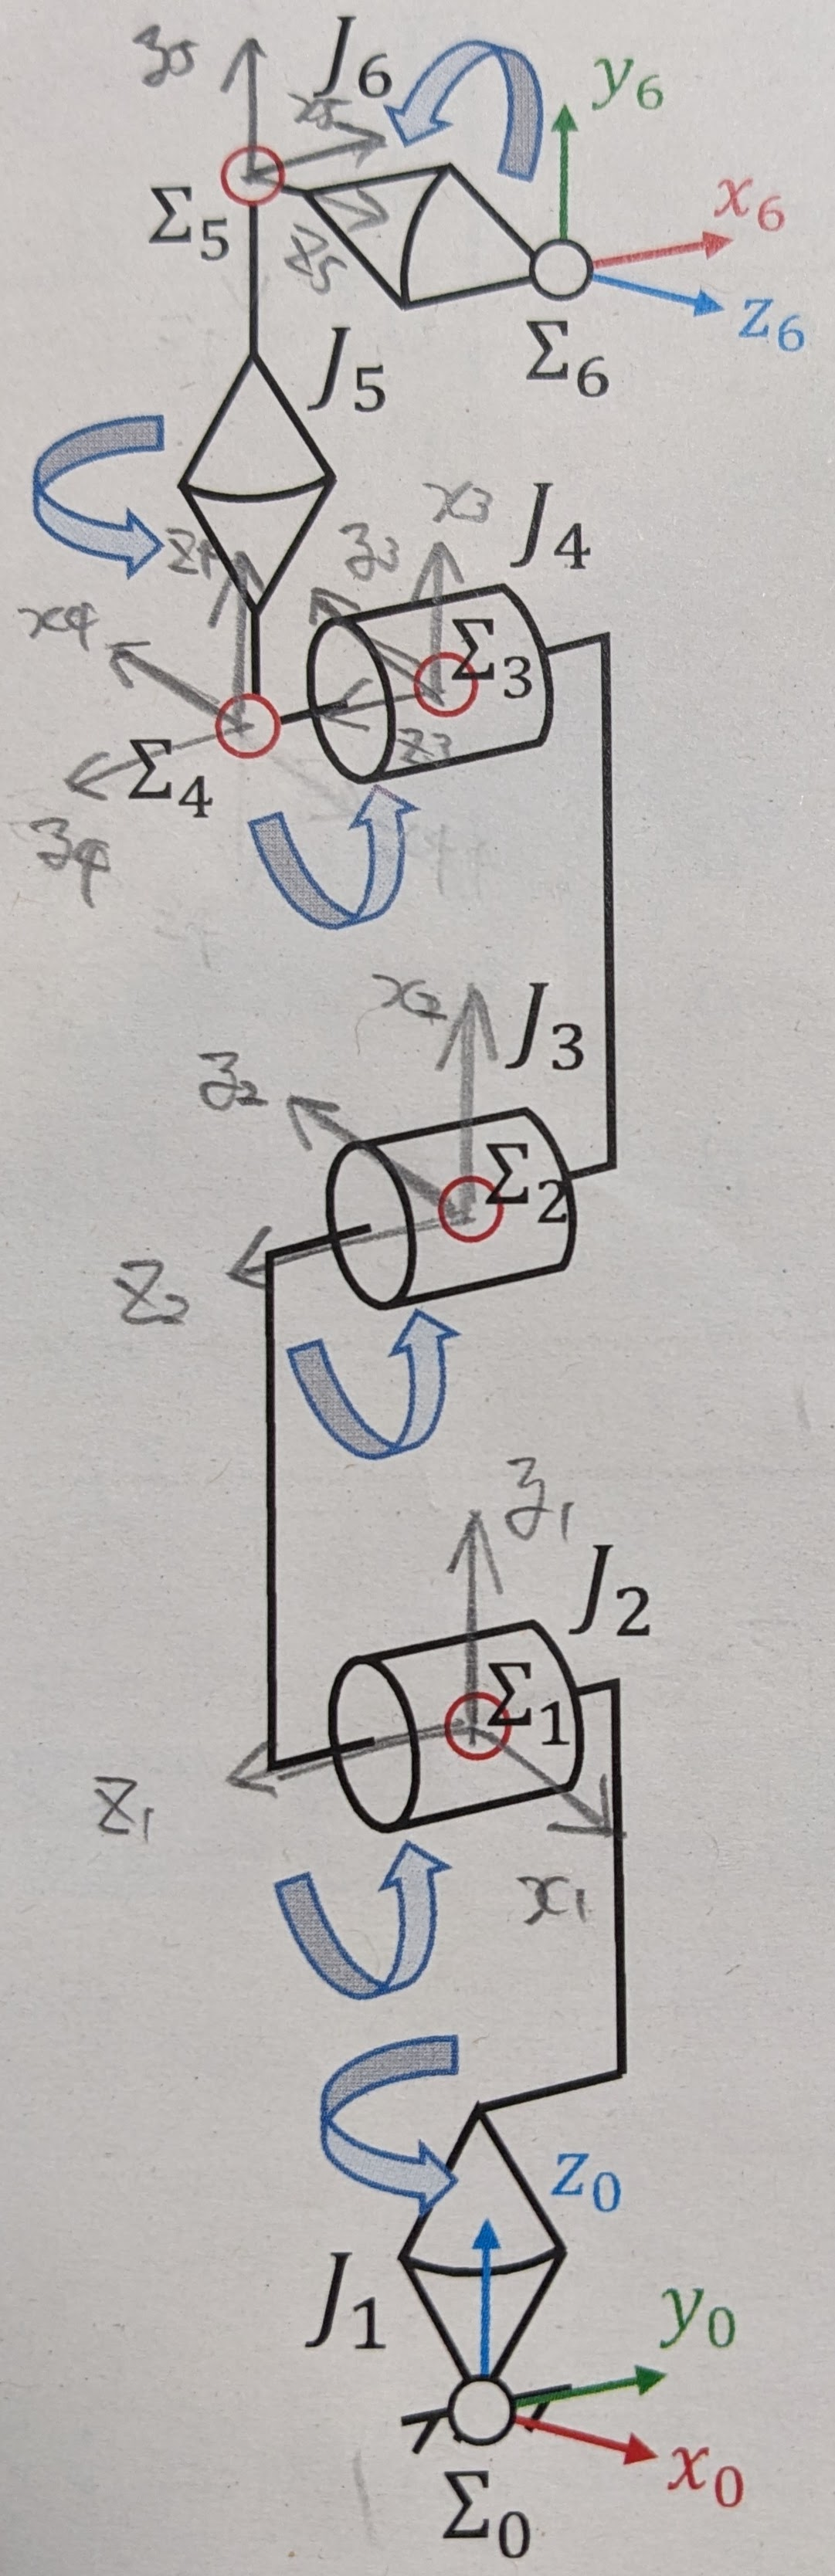
\includegraphics[width = 0.7\linewidth]{../results/robot_arm_DH.jpg}
			\subcaption{DH法により座標系を定義}
			\label{fig:ロボットアームのモデルと座標系-DH法により座標系を定義}
		\end{minipage}
	\end{tabular}
	\caption{ロボットアームのモデルと座標系}
	\label{fig:ロボットアームのモデルと座標系}
\end{figure}

\subsection{リンクパラメータを求め同次変換行列$^{i-1}T_i$を定義}
座標系$\Sigma_{i-1}$から$\Sigma_i$へ移動するときの関係を記述する同次変換行列$^{i-1}T_i$を定義する.$i-1$から$i$への移動は次のように行う.
\begin{enumerate}
	\item $z_{i-1}$軸方向に$d_i$並進
	\item $z_{i-1}$軸まわりに$\theta_i$回転
	\item $x_i$軸方向に$l_i$並進
	\item $x_i$軸回りに$\alpha_i$回転
\end{enumerate}
$i-1$から$i$への移動をこのように定義した場合,同次変換行列$^{i-1}T_i$は\cref{eq:同次変換行列}となる.
\begin{align}
	\label{eq:同次変換行列}
	\mqty[
		\cos \theta_i & -\cos \alpha_i \sin \theta_i & \sin \alpha_i \sin \theta_i & l_i \cos \theta_i \\
		\sin \theta_i & \cos \alpha_i \cos \theta_i & -\sin \alpha_i \cos \theta_i & l_i \sin \theta_i \\
		0 & \sin \alpha_i & \cos \alpha_i & d_i \\
		0 & 0 & 0 & 1 \\
	]
\end{align}

まずはロボットアームのリンクパラメータを求める.\cref{tab:リンクパラメータ}に示す.
\begin{table}[H]
	\centering
	\caption{リンクパラメータ}
	\label{tab:リンクパラメータ}
	\begin{tblr}{
		cells = {halign = r, mode=dmath},
		hline{1,Z} = {0.08em},
		hline{2} = {0.04em}
	}
		^{i-1}T_i & d_i & \theta_i & l_i & \alpha_i \\
		^0T_1 & d_1 & \theta_1 & 0 & \cfrac{\pi}{2} \\
		^1T_2 & 0 & \theta_2 & l_2 & 0 \\
		^2T_3 & 0 & \theta_3 & l_3 & 0 \\
		^3T_4 & d_4 & \theta_4 & 0 & \cfrac{\pi}{2} \\
		^4T_5 & d_5 & \theta_5 & 0 & \cfrac{\pi}{2} \\
		^5T_6 & d_6 & \theta_6 & 0 & 0 \\
	\end{tblr}
\end{table}

\cref{tab:リンクパラメータ}を\cref{eq:同次変換行列}に代入し,$^{i-1}T_i$を求めた.\cref{eq:0T1,eq:1T2,eq:2T3,eq:3T4,eq:4T5,eq:5T6}に示す.ただし,$C_i \coloneqq \cos \theta_i, S_i \coloneqq \sin \theta_i$である.
\begin{align}
	\label{eq:0T1}
	^0T_1 &= \mqty[
		C_1 & 0 & S_1 & 0 \\
		S_1 & 0 & -C_1 & 0 \\
		0 & 1 & 0 & d_1 \\
		0 & 0 & 0 & 1 
	]
	\\
	\label{eq:1T2}
	^1T_2 &= \mqty[
		C_2 & -S_2 & 0 & l_2 C_2 \\
		S_2 & C_2 & 0 & l_2 S_2 \\
		0 & 0 & 1 & 0 \\
		0 & 0 & 0 & 1 
	]
	\\
	\label{eq:2T3}
	^2T_3 &= \mqty[
		C_3 & -S_3 & 0 & l_3 C_3 \\
		S_3 & C_3 & 0 & l_3 S_3 \\
		0 & 0 & 1 & 0 \\
		0 & 0 & 0 & 1 
	]
	\\
	\label{eq:3T4}
	^3T_4 &= \mqty[
		C_4 & 0 & S_4 & 0 \\
		S_4 & 0 & -C_4 & 0 \\
		0 & 1 & 0 & d_4 \\
		0 & 0 & 0 & 4 
	]
	\\
	\label{eq:4T5}
	^4T_5 &= \mqty[
		C_5 & 0 & S_5 & 0 \\
		S_5 & 0 & -C_5 & 0 \\
		0 & 1 & 0 & d_5 \\
		0 & 0 & 0 & 5 
	]
	\\
	\label{eq:5T6}
	^5T_6 &= \mqty[
		C_6 & -S_6 & 0 & 0 \\
		S_6 & C_6 & 0 & 0 \\
		0 & 0 & 1 & d_6 \\
		0 & 0 & 0 & 1
	]
\end{align}

\subsection{DH法における角度$\theta_i$とサーボモータの角度$J_i$の対応付け}
DH法における角度$\theta_i$は$x_{i-1}$軸と$x_i$軸のなす角であるのに対し,ロボットの関節に搭載されているサーボモータの角度$J_i$は\cref{fig:ロボットアームのモデルと座標系}の直立姿勢において$J_i = 0, i = 1 \dots 6$である.また,$\theta_i$が弧度法なのに対し,$J_i$は分度法である.この異なる定義の角度$\theta_i$と$J_i$の対応付けを行った.\cref{eq:theta1-J1,eq:theta2-J2,eq:theta3-J3,eq:theta4-J4,eq:theta5-J5,eq:theta6-J6}に示す.
\begin{align}
	\label{eq:theta1-J1}
	\theta_1 &= \cfrac{J_1}{180} \pi + 0 \\
	\label{eq:theta2-J2}
	\theta_2 &= \cfrac{J_2}{180} \pi + \cfrac{\pi}{2} \\
	\label{eq:theta3-J3}
	\theta_3 &= \cfrac{J_3}{180} \pi + 0 \\
	\label{eq:theta4-J4}
	\theta_4 &= \cfrac{J_4}{180} \pi + \cfrac{\pi}{2} \\
	\label{eq:theta5-J5}
	\theta_5 &= \cfrac{J_5}{180} \pi - \cfrac{\pi}{2} \\
	\label{eq:theta6-J6}
	\theta_6 &= \cfrac{J_6}{180} \pi + 0
\end{align}

\subsection{座標系$\Sigma_0$基準でのアーム手先位置を求める順運動学問題}
手先の位置は,$\Sigma_6$基準では$^6p_t = \mqty[0 & 0 & 0 & 1]^\mathsf{T}$である.これに対して\cref{eq:0T1,eq:1T2,eq:2T3,eq:3T4,eq:4T5,eq:5T6}の同次変換行列を左から順にかけていくことにより,$\Sigma_0$基準の手先位置$^0p_t$が\cref{eq:手先座標-順運動学-計算済み}のように求まる.導出過程を\cref{eq:手先座標-順運動学,eq:手先座標-順運動学-途中式,eq:手先座標-順運動学-計算済み}に示す.なお,\cref{eq:手先座標-順運動学}の行列の積の展開にはSympyを用いた.
\begin{align}
	\label{eq:手先座標-順運動学}
	^0p_t &= ^0T_1 ^1T_2 ^2T_3 ^3T_4 ^4T_5 ^5T_6 ^6p_t \\
	\label{eq:手先座標-順運動学-途中式}
	&= \mqty[
		C_1C_2C_3l_3 - C_1S_2S_3 + C_1C_2l_2 + C_1d_5(C_4S_{23} + S_4C_{23}) + S_1d_4 - d_6\qty{-C_1S_5(C_4C_{23} - S_4S_{23}) + S_1C_5} \\
		S_1C_2C_3l_3 - S_1S_2S_3 + S_1C_2l_2 + C_1d_5(C_4S_{23} + S_4C_{23}) - C_1d_4 - d_6\qty{S_1S_5(C_4C_{23} - S_4S_{23}) + C_1C_5} \\
		C_2S_3l_3 + S_2C_3l_3 + S_5d_6(C_4S_{23} + S_4C_{23}) + d_1 - d_5(C_4S_{23} - S_4S_{23}) \\
		1
	]
	\\
	\label{eq:手先座標-順運動学-計算済み}
	&= \mqty[
		(d_5S_4 + d_6C_4S_5)C_1C_{23} + (d_5C_4 - d_6S_4S_5)C_1S_{23} + (l_2 + l_3C_3)C_1C_2 + (d_4 - d_6C_5)S_1 - l_3C_1S_2S_3 \\
		(d_5S_4 + d_6C_4S_5)S_1S_{23} + (d_5C_4 - d_6S_4S_5)S_1S_{23} + (l_2 + l_3C_3)S_1C_2 + (d_4 - d_6C_5)C_1 - l_3S_1S_2S_3 \\
		(d_5S_4 + d_6C_4S_5)S_{23} + (d_5C_4 - d_6S_4S_5)C_{23} + (l_2 + l_3C_3)S_2 + d_1 + l_3C_2S_3 \\
		1
	]
\end{align}

\subsection{6関節角度を入力し,全関節を同時に動作させるプログラムの作成}\label{subsec:6関節角度を入力し,全関節を同時に動作させるプログラム}
sample.pyを書き換えることにより,6関節角度を入力し,全関節を同時に動作させるプログラムを作成した.実際に作成したプログラムは付録のListing \ref{src:6関節角度を入力し,全関節を同時に動作させるプログラム}に掲載しておく.

6関節角度に$\bm{J} = \mqty[-12.08 & -51.17 & -123.8 & 84.96 & 0.0 & -12.08]^\mathsf{T}$を与えたときのシミュレーション結果を\cref{fig:6関節角度に-を与えたときのロボットの形状}に示す.
\begin{figure}[H]
	\centering
	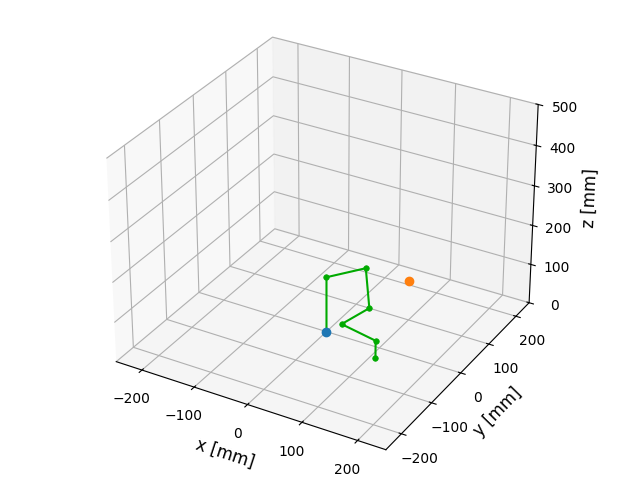
\includegraphics[width = 0.5\linewidth]{../results/program2.png}
	\caption{6関節角度に$\bm{J} = \mqty[-12.08 & -51.17 & -123.8 & 84.96 & 0.0 & -12.08]^\mathsf{T}$を与えたときのロボットの形状}
	\label{fig:6関節角度に-を与えたときのロボットの形状}
\end{figure}

\subsection{順運動学により,関節角度から手先位置を計算するプログラムの作成}\label{subsec:順運動学により,関節角度から手先位置を計算するプログラムの作成}
\cref{eq:手先座標-順運動学-計算済み}に示した順運動学の式を使い,関節角度から手先位置を計算するプログラムを作成した.実際に作成したプログラムは付録のListing \ref{src:順運動学により,関節角度から手先位置を計算するプログラムの作成}に掲載しておく.

次の関節角度と手先位置の組の例について,関節角度をシミュレータに入力し,手先位置の同次座標が正しく出力されること,マーカ位置と手先位置が一致することを確認した.コマンドラインの出力については以下に,シミュレーション結果の画像出力については\cref{fig:順運動学から計算した手先位置}に示す.
\begin{enumerate}[label=(\alph*)]
	\item $\bm{J} = \mqty[-12.08 & -51.17 & -123.8 & 84.96 & 0.0 & -12.08]^\mathsf{T}, ^0p_t = \mqty[150 & -100 & 70 & 1]^\mathsf{T}$ \\ 
	出力された同次座標
	\begin{lstlisting}
		[149.98707521 -99.99309332  69.97903252   1.        ]
	\end{lstlisting}
	\item $\bm{J} = \mqty[-34.7 & -63.36 & -119.18 & 92.54 & 0.0 & -34.7]^\mathsf{T}, ^0p_t = \mqty[100 & -150 & 50 & 1]^\mathsf{T}$ \\
	出力された同次座標
	\begin{lstlisting}
		[ 100.00154038 -149.99662236   49.99582456    1.        ]
	\end{lstlisting}
	\item $\bm{J} = \mqty[26.27 & -26.46 & -146.28 & 82.74 & 0.0 & 26.27]^\mathsf{T}, ^0p_t = \mqty[150 & 0 & 100 & 1]^\mathsf{T}$ \\
	出力された同次座標
	\begin{lstlisting}
		[ 1.49995606e+02 -1.87934829e-03  1.00004760e+02  1.00000000e+00]
	\end{lstlisting}
	\item $\bm{J} = \mqty[55.30 & -51.17 & -123.80 & 84.96 & 0.0 & 55.30]^\mathsf{T}, ^0p_t = \mqty[150 & 100 & 70 & 1]^\mathsf{T}$ \\
	出力された同次座標
	\begin{lstlisting}
		[149.98888922  99.9903723   69.97903252   1.        ]
	\end{lstlisting}
	\item $\bm{J} = \mqty[77.92 & -63.36 & -119.18 & 92.54 & 0.0 & 77.92]^\mathsf{T}, ^0p_t = \mqty[100 & 150 & 50 & 1]^\mathsf{T}$ \\
	出力された同次座標
	\begin{lstlisting}
		[ 99.99593616 150.0003585   49.99582456   1.        ]
	\end{lstlisting}
\end{enumerate}

\begin{figure}[H]
	\centering
	\begin{tabular}{cc}
		\begin{minipage}[c]{0.48\linewidth}
			\centering
			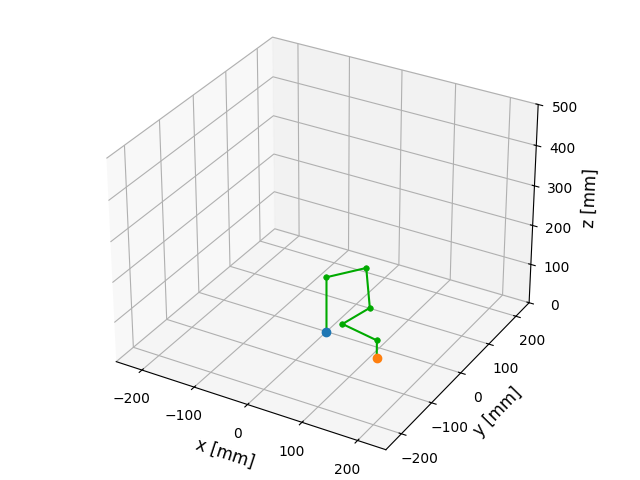
\includegraphics[width = 0.96\linewidth]{../results/program3_1.png}
			\subcaption{}
		\end{minipage}
		&
		\begin{minipage}[c]{0.48\linewidth}
			\centering
			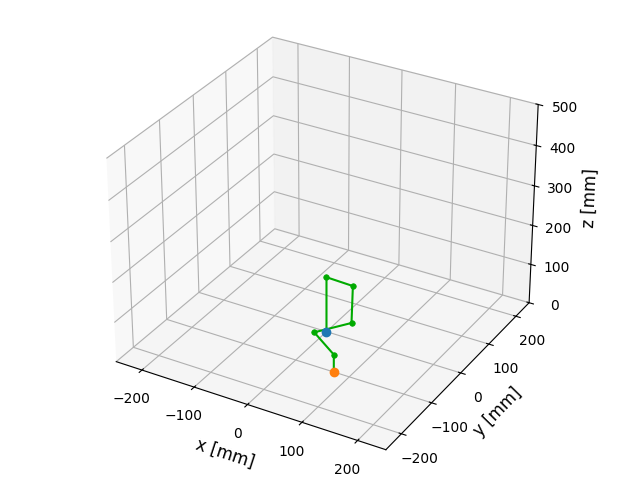
\includegraphics[width = 0.96\linewidth]{../results/program3_2.png}
			\subcaption{}
		\end{minipage}
		\\
		\begin{minipage}[c]{0.48\linewidth}
			\centering
			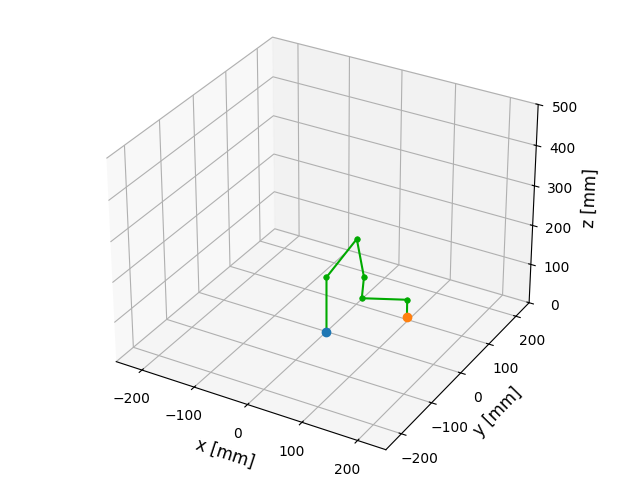
\includegraphics[width = 0.96\linewidth]{../results/program3_3.png}
			\subcaption{}
		\end{minipage}
		&
		\begin{minipage}[c]{0.48\linewidth}
			\centering
			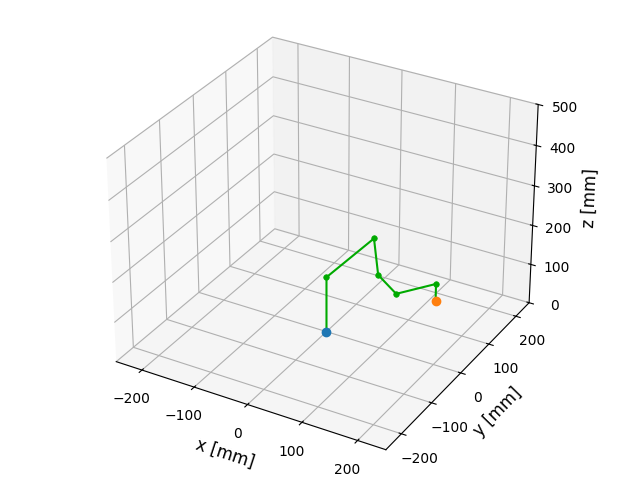
\includegraphics[width = 0.96\linewidth]{../results/program3_4.png}
			\subcaption{}
		\end{minipage}
		\\
		\begin{minipage}[c]{0.48\linewidth}
			\centering
			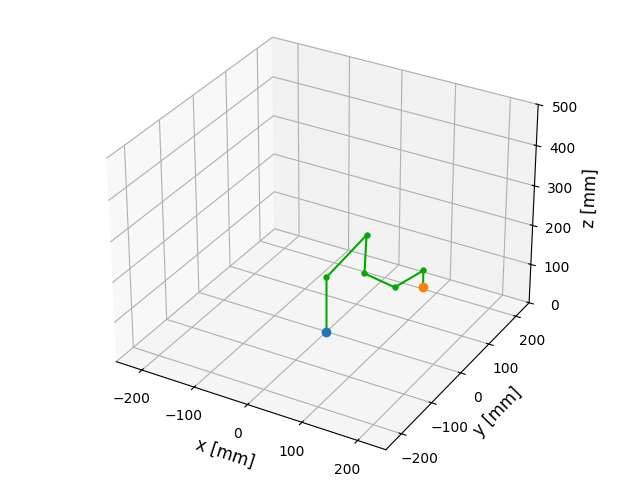
\includegraphics[width = 0.96\linewidth]{../results/program3_5.png}
			\subcaption{}
		\end{minipage}
		& \\
	\end{tabular}
	\caption{順運動学から計算した手先位置}
	\label{fig:順運動学から計算した手先位置}
\end{figure}

\subsection{$Z$方向の手先位置が\SI{15}{\mm}以内の場合にエラーを発生させるプログラム}\label{subsec:Z方向の手先位置が15mm以内の場合にエラーを発生させるプログラム}
\cref{subsec:順運動学により,関節角度から手先位置を計算するプログラムの作成}に対して,$Z$方向の手先位置が\SI{15}{\mm}以内の場合にZ\_ERRORを発生させるようにした.実際に作成したプログラムは付録のListing \ref{src:Z方向の手先位置が15mm以内の場合にエラーを発生させるプログラム}に掲載しておく.

次の関節角度と手先位置の組の例について,関節角度をシミュレータに入力し,(a)については正しく同次座標が求まること,(b)-(d)についてはエラーが出ることを確認した.その結果を以下に示す.
\begin{enumerate}[label=(\alph*)]
	\item $\bm{J} = \mqty[63.24 & -41.72 & -103.45 & 55.17 & 0.0 & 63.24]^\mathsf{T}, ^0p_t = \mqty[150 & 150 & 100 & 1]^\mathsf{T}$ \\
	出力された同次座標
	\begin{lstlisting}
		[149.99687637 150.00915832 100.00158833   1.        ]^\mathsf{T}
	\end{lstlisting}
	\item $\bm{J} = \mqty[63.24 & -85.92 & -83.17 & 79.09 & 0.0 & 63.24]^\mathsf{T}, ^0p_t = \mqty[150 & 150 & 10 & 1]^\mathsf{T}$ \\
	出力されたエラー
	\begin{lstlisting}
		ZError: z error
	\end{lstlisting}
	\item $\bm{J} = \mqty[145.3 & -63.36 & -119.18 & 92.54 & 0.0 & 145.3]^\mathsf{T}, ^0p_t = \mqty[-100 & 150 & 50 & 1]^\mathsf{T}$ \\
	出力されたエラー
	\begin{lstlisting}
		AngleError: J1 angle error
	\end{lstlisting}
	\item $\bm{J} = \mqty[41.6 & -118.04 & -155.24 & 183.28 & 0.0 & 41.6]^\mathsf{T}, ^0p_t = \mqty[100 & 50 & 50 & 1]^\mathsf{T}$ \\
	出力されたエラー
	\begin{lstlisting}
		AngleError: J3 angle error
	\end{lstlisting}
\end{enumerate}

\subsection{実機で\cref{subsec:Z方向の手先位置が15mm以内の場合にエラーを発生させるプログラム}のプログラムの動作を確認}
実機で\cref{subsec:Z方向の手先位置が15mm以内の場合にエラーを発生させるプログラム}のプログラム(Listing \ref{src:Z方向の手先位置が15mm以内の場合にエラーを発生させるプログラム})の動作を確認した.

\cref{subsec:順運動学により,関節角度から手先位置を計算するプログラムの作成}の角度例を入力すると,実機においてもシミュレータと同じ手先位置・形状になることが確認できた.また,\cref{subsec:Z方向の手先位置が15mm以内の場合にエラーを発生させるプログラム}の角度例を入力すると,実機においても同じエラーが出力され,エラーの場合はロボットが動作しないことを確認できた.

\subsection{関節角度間の関係に拘束条件を与えた場合の順運動学}\label{subsec:関節角度間の関係に拘束条件を与えた場合の順運動学}
\begin{figure}[H]
	\centering
	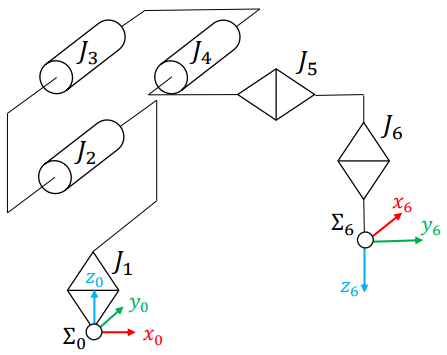
\includegraphics[width = 0.75\linewidth]{../figures/robot_arm_constraints.png}
	\caption{関節角度間の拘束条件}
	\label{fig:関節角度間の拘束条件}
\end{figure}

\cref{fig:関節角度間の拘束条件}に示すような拘束条件を与え,順運動学を簡略化する.\cref{fig:関節角度間の拘束条件}の拘束条件を表す式は\cref{eq:拘束条件-theta4,eq:拘束条件-theta5,eq:拘束条件-theta6}である.
\begin{align}
	\label{eq:拘束条件-theta4}
	\theta_4 &= \cfrac{\pi}{2} - \theta_2 - \theta_3 \\
	\label{eq:拘束条件-theta5}
	\theta_5 &= -\cfrac{\pi}{2} \\
	\label{eq:拘束条件-theta6}
	\theta_6 &= \theta_1
\end{align}

\cref{eq:拘束条件-theta4,eq:拘束条件-theta5,eq:拘束条件-theta6}の条件を与えたとき,\cref{eq:手先座標-順運動学-計算済み}に示した手先位置は\cref{eq:手先座標-順運動学-拘束}となる.
\begin{align}
	\label{eq:手先座標-順運動学-拘束}
	^0p_t = \mqty[
		l_3C_1C_2C_3 - l_3C_1S_2S_3 + l_2C_1C_2 + d_4S_1 + d_5C_1 \\
		l_3S_1C_2C_3 - l_3S_1S_2S_3 + l_2S_1C_2 - d_4C_1 + d_5S_1 \\
		l_3C_2S_3 + l_3S_2C_3 + l_2S_2 + d_1 - d_6 \\
		1
	]
\end{align}

\subsection{手先位置が与えられたときの$\theta_1$を求める}\label{subsec:手先位置が与えられたときのtheta1を求める}
\begin{figure}[H]
	\centering
	\begin{tabular}{cc}
		\begin{minipage}[c]{0.48\linewidth}
			\centering
			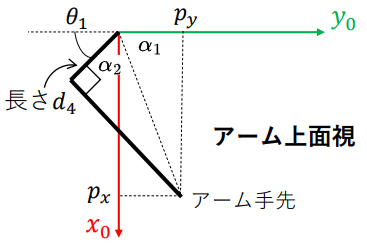
\includegraphics[width = 0.96\linewidth]{../figures/figures-theta1_py>0_edit.drawio.png}
			\subcaption{$p_y > 0$}
			\label{fig:py>0}
		\end{minipage}
		&
		\begin{minipage}[c]{0.48\linewidth}
			\centering
			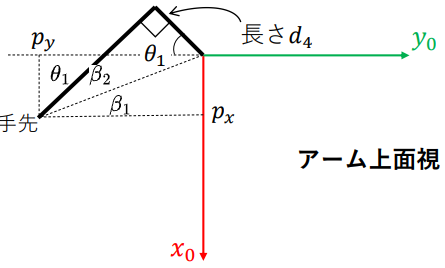
\includegraphics[width = 0.96\linewidth]{../figures/figures-theta1_py<=0_edit.drawio.png}
			\subcaption{$p_y \leq 0$}
			\label{fig:py<=0}
		\end{minipage}
	\end{tabular}
	\caption{$p_y$で場合分けした$\theta_1$}
	\label{fig:pyで場合分けしたtheta1}
\end{figure}

手先位置$\mqty[p_x & p_y & p_z]^\mathsf{T}$が与えられたときの$\theta_1$を求める.$p_y$で場合分けすると,\cref{fig:pyで場合分けしたtheta1}のようになる.それぞれの場合について$\theta_1$を求めていく.

まず,$p_y > 0$の場合について考える.\cref{fig:py>0}のように角度$\alpha_1, \alpha_2$を定義する.$\alpha_1, \alpha_2$はそれぞれ\cref{eq:py>0-alpha1,eq:py>0-alpha2}となる.
\begin{align}
	\label{eq:py>0-alpha1}
	\alpha_1 &= \text{atan2}(p_x, p_y) \\
	\label{eq:py>0-alpha2}
	\alpha_2 &= \cos^{-1}\qty(\cfrac{d_4}{\sqrt{p_x^2 + p_y^2}})
\end{align}
よって,$\theta_1 (p_y > 0)$が\cref{eq:py>0-theta1}のように求まる.
\begin{align}
	\theta_1 &= \pi - \alpha_1 - \alpha_2 \\
	\label{eq:py>0-theta1}
	&= \pi - \text{atan2}(p_x, p_y) - \cos^{-1}\qty(\cfrac{d_4}{\sqrt{p_x^2 + p_y^2}})
\end{align}

次に,$p_y \leq 0$の場合について考える.\cref{fig:py<=0}のように角度$\beta_1, \beta_2$を定義する.$p_y \leq 0$であることに注意すると,$\beta_1, \beta_2$はそれぞれ\cref{eq:py<=0-beta1,eq:py<=0-beta2}となる.
\begin{align}
	\label{eq:py<=0-beta1}
	\beta_1 &= \sin^{-1}\qty(\cfrac{d_4}{\sqrt{p_x^2 + p_y^2}}) \\
	\label{eq:py<=0-beta2}
	\beta_2 &= \text{atan2}(-p_y, p_x) \\
\end{align}
よって,$\theta_1 (p_y \leq 0)$が\cref{eq:py<=0-theta1}のように求まる.
\begin{align}
	\theta_1 &= \cfrac{\pi}{2} - \beta_1 - \beta_2 \\
	\label{eq:py<=0-theta1}
	&= \cfrac{\pi}{2} - \text{atan2}(-p_y, p_x) - \sin^{-1}\qty(\cfrac{d_4}{\sqrt{p_x^2 + p_y^2}})
\end{align}

したがって,\cref{eq:py>0-theta1,eq:py<=0-theta1}より,$\theta_1$は\cref{eq:theta1}のように求まる.
\begin{align}
	\label{eq:theta1}
	\theta_1 = 
	\begin{cases}
		\pi - \text{atan2}(p_x, p_y) - \cos^{-1}\qty(\cfrac{d_4}{\sqrt{p_x^2 + p_y^2}}) & \text{if}\,p_y > 0 \\
		\cfrac{\pi}{2} - \text{atan2}(-p_y, p_x) - \sin^{-1}\qty(\cfrac{d_4}{\sqrt{p_x^2 + p_y^2}}) & \text{if}\,p_y \leq 0
	\end{cases}
\end{align}

\subsection{手先位置が与えられたときの$\theta_2, \theta_3$を求める}\label{subsec:手先位置が与えられたときのtheta2,theta3を求める}
手先位置$\mqty[p_x & p_y & p_z]^\mathsf{T}$が与えられたときの$\theta_2,\theta_3$を求める.

\cref{eq:手先座標-順運動学-拘束}より,
\begin{align}
	\label{eq:px-pz}
	&\mqty[p_x \\ p_z] = \mqty[
		l_3C_1C_3 + l_2C_1 & -l_3C_1S_3 \\
		l_3S_3 & l_3C_3 + l_2
	]
	\mqty[C_2 \\ S_2]
	+
	\mqty[d_5C_1 + d_4S_1 \\ d_1 - d_6] \\
	\label{eq:px-pz-変形}
	\therefore
	&\mqty[\cfrac{p_x - d_4S_1 - d_5C_1}{C_1} \\ p_z - d_1 + d_6]
	=
	\mqty[
		l_3C_3 + l_2 & -l_3S_3 \\
		l_3S_3 & l_3C_3 + l_2
	]
	\mqty[C_2 \\ S_2]
\end{align}
\cref{eq:px-pz-変形}の左辺を極座標形式で表現する.
\begin{align}
	\label{eq:def-pxp-pzp}
	\mqty[p_x' \\ p_z'] \coloneqq \mqty[\cfrac{p_x - d_4S_1 - d_5C_1}{C_1} \\ p_z - d_1 + d_6] \\
	\label{eq:左辺-極座標}
	\text{(左辺)} = \sqrt{p_x'^2 + p_z'^2} \mqty[\cos\alpha \\ \sin\alpha] \\
\end{align}
ただし,$\alpha$は,
\begin{align}
	\label{eq:def-alpha}
	\alpha \coloneqq \text{atan2}(p_z', p_x')
\end{align}
\cref{eq:px-pz-変形}の右辺を極座標形式で表現する.
\begin{align}
	\text{(右辺)} &=
	\sqrt{l_2^2 + l_3^2 + 2l_2l_3C_3} \mqty[
		\cos\beta & -\sin\beta \\
		\sin\beta & \cos\beta
	]
	\mqty[C_2 \\ S_2] \\
	\label{eq:右辺-極座標}
	&= \sqrt{l_2^2 + l_3^2 + 2l_2l_3C_3} \mqty[\cos(\theta_2 + \beta) \\ \sin(\theta_2 + \beta)]
\end{align}
ただし,$\beta$は
\begin{align}
	\label{eq:def-beta}
	\beta \coloneqq \text{atan2}(l_3S_3, l_3C_3 + l_2)
\end{align}

以上より,
\begin{align}
	p_x'^2 + p_z'^2 = l_2^2 + l_3^2 + 2l_2l_3C_3 \\
	\therefore
	C_3 = \cfrac{p_x'^2 + p_z'^2 - l_2^2 + l_3^2}{2l_2l_3C_3} \\
	\label{eq:theta3}
	\therefore
	\theta_3 = \pm\text{atan2}(\sqrt{1 - C_3^2}, C_3)
\end{align}
\begin{align}
	\theta_2 &= \alpha - \beta \\
	\label{eq:theta2}
	&= \text{atan2}(p_z', p_x') - \text{atan2}(l_3S_3, l_3C_3 + l_2)
\end{align}

\subsection{逆運動学により入力した位置に手先を移動させるプログラムを作成}\label{subsec:逆運動学により入力した位置に手先を移動させるプログラムを作成}
逆運動学により入力した位置に手先を移動させるプログラムを作成し,シミュレータ上で動作を確認した.作成したプログラムは付録のListing \ref{src:逆運動学により入力した位置に手先を移動させるプログラム}に掲載しておく.

\cref{eq:theta3}の$\theta_3$の計算において,atan2の符号は$-$とした.また,atan2とsqrtの実行前に,これらの関数が計算可能化を判定し,計算不可の場合はそれぞれエラーが発生するようにした.

エラーについて,atan2の場合は分母の絶対値が$0.001$以下になる場合,ZeroDivisionErrorをraiseするようにした.sqrtの場合,根号の中身が負になった場合,SqrtErrorをraiseするようにした.

次の4つの手先位置を与え,シミュレータの動作を確認した.(a),(b)は動作範囲内かつエラーも出ない適切な手先位置である.これら2つの手先位置を与えた場合のロボットアームのシミュレーション上の挙動を\cref{fig:適切な手先位置が与えられたときのロボットアームの挙動}に示す.(c)はatan2の分母のゼロ割り,(d)はsqrtの中身が負になることを意図して設定した.それぞれの場合に出力されたエラーを以下に示す.
\begin{enumerate}[label=(\alph*)]
	\item $^0p_t = \mqty[150 & -100 & 70 & 1]^\mathsf{T}$
	\item $^0p_t = \mqty[100 & -150 & 50 & 1]^\mathsf{T}$
	\item $^0p_t = \mqty[0 & 0 & 100 & 1]^\mathsf{T}$ \\
	\begin{lstlisting}
		ZeroDivisionError: zero_division error
	\end{lstlisting}
	\item $^0p_t = \mqty[1000 & 1000 & 100 & 1]^\mathsf{T}$ \\
	\begin{lstlisting}
		SqrtError: sqrt error
	\end{lstlisting}
\end{enumerate}

\begin{figure}[H]
	\centering
	\begin{tabular}{cc}
		\begin{minipage}[c]{0.48\linewidth}
			\centering
			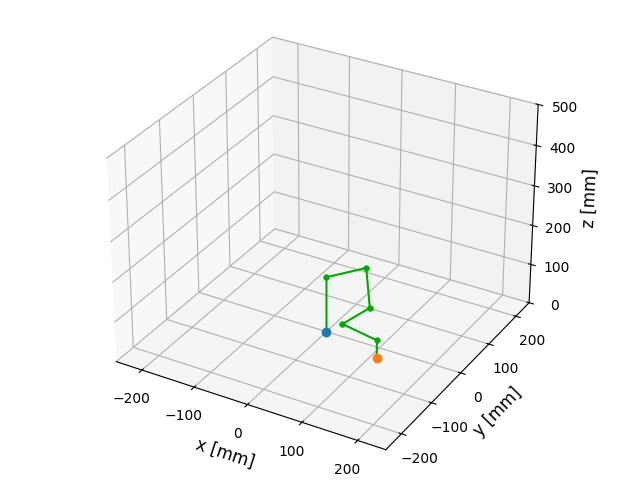
\includegraphics[width = 0.96\linewidth]{../results/program7_1.png}
			\subcaption{}
		\end{minipage}
		&
		\begin{minipage}[c]{0.48\linewidth}
			\centering
			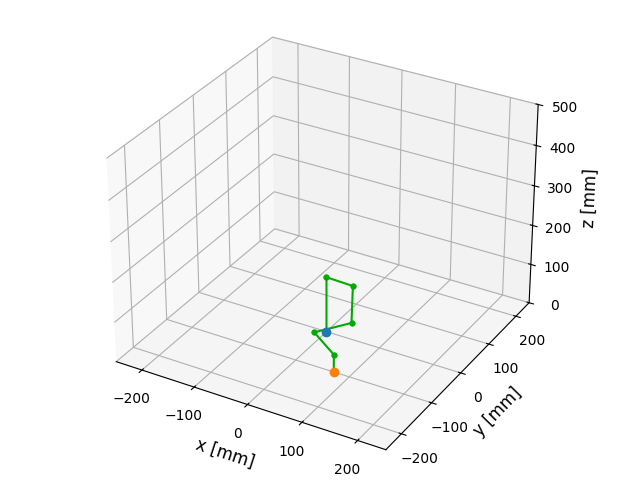
\includegraphics[width = 0.96\linewidth]{../results/program7_2.png}
			\subcaption{}
		\end{minipage}
	\end{tabular}
	\caption{適切な手先位置が与えられたときのロボットアームの挙動}
	\label{fig:適切な手先位置が与えられたときのロボットアームの挙動}
\end{figure}

\subsection{初期位置にあるプレートを最終位置に移動させるプログラム}\label{subsec:初期位置にあるプレートを最終位置に移動させるプログラム}
初期位置にあるプレートを最終位置に移動させるプログラムを作成した.作成したプログラムは付録のListing \ref{src:初期位置にあるプレートを最終位置に移動させるプログラム}に掲載しておく.

今回は初期位置を$^0p_t = \mqty[150 & -100 & 50 & 1]^\mathsf{T}$,最終位置を$^0p_t = \mqty[100 & -150 & 50 & 1]^\mathsf{T}$とした.運搬のときは,$z$軸方向に\SI{100}{\mm}だけ持ち上げてから運搬するようにした.そのため,運搬時の軌跡は初期位置と最終位置,それからそれらの上空\SI{100}{\mm}の位置を結んだコの字型になる.
基本的には\cref{subsec:逆運動学により入力した位置に手先を移動させるプログラムを作成}を4回繰り返すようにして実装した.

シミュレーション上での初期位置から最終位置までの運搬のようすを\cref{fig:初期位置から最終位置までの運搬のようす-シミュレーション}に示す.
\begin{figure}[H]
	\centering
	\begin{tabular}{cc}
		\begin{minipage}[c]{0.48\linewidth}
			\centering
			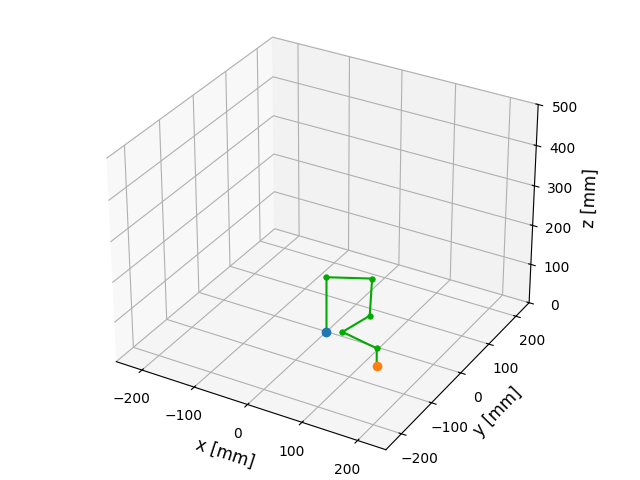
\includegraphics[width = 0.96\linewidth]{../results/program8_1.png}
			\subcaption{初期位置$\mqty[150 & -100 & 50 & 1]^\mathsf{T}$}
		\end{minipage}
		&
		\begin{minipage}[c]{0.48\linewidth}
			\centering
			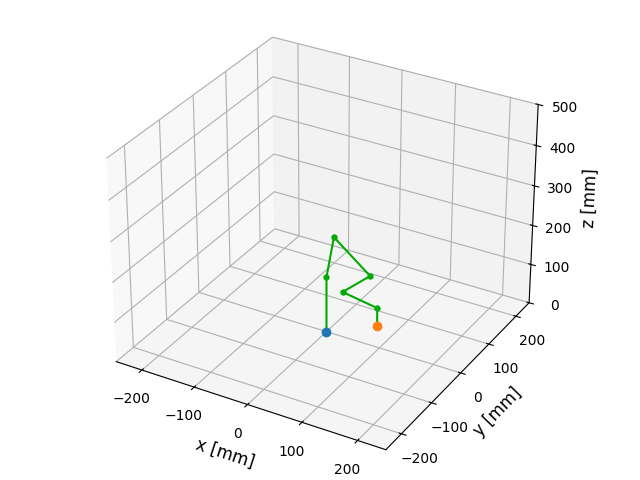
\includegraphics[width = 0.96\linewidth]{../results/program8_2.png}
			\subcaption{初期位置上空$\mqty[150 & -100 & 150 & 1]^\mathsf{T}$}
		\end{minipage}
		\\
		\begin{minipage}[c]{0.48\linewidth}
			\centering
			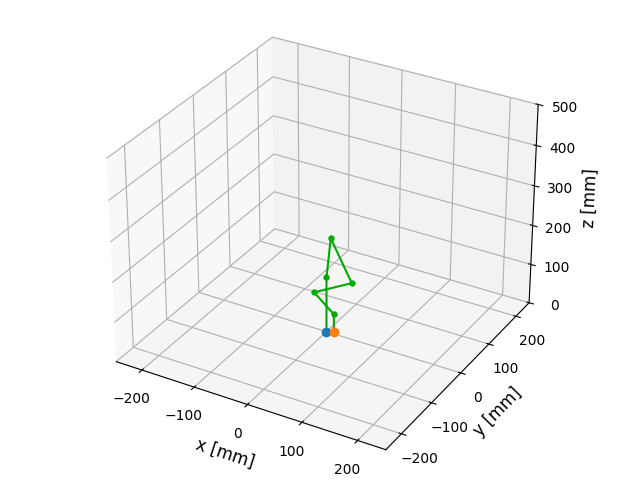
\includegraphics[width = 0.96\linewidth]{../results/program8_3.png}
			\subcaption{最終位置上空$\mqty[100 & -150 & 150 & 1]^\mathsf{T}$}
		\end{minipage}
		&
		\begin{minipage}[c]{0.48\linewidth}
			\centering
			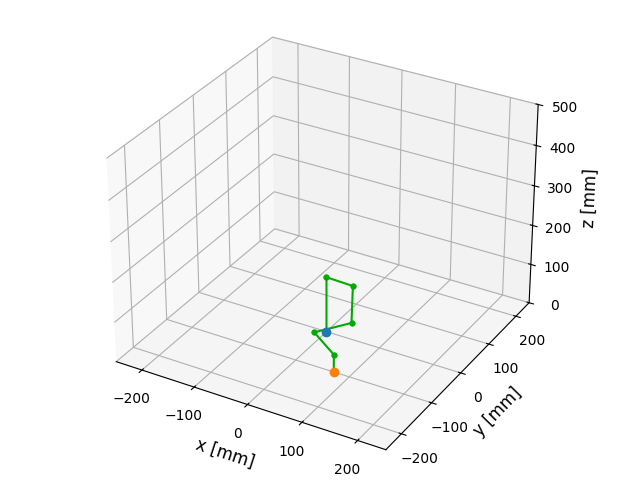
\includegraphics[width = 0.96\linewidth]{../results/program8_4.png}
			\subcaption{最終位置$\mqty[100 & -150 & 50 & 1]^\mathsf{T}$}
		\end{minipage}
	\end{tabular}
	\caption{初期位置から最終位置までの運搬のようす(シミュレーション)}
	\label{fig:初期位置から最終位置までの運搬のようす-シミュレーション}
\end{figure}

\subsection{\cref{subsec:初期位置にあるプレートを最終位置に移動させるプログラム}を実機にて動作確認}
\cref{subsec:初期位置にあるプレートを最終位置に移動させるプログラム}において作成したプログラムを実機で実行し,動作を確認した.また,運搬中の状態が視覚的にわかりやすいように,ロボットアーム付属のLEDを初期位置から順に赤,緑,青,白で点灯するようにした.作成したプログラムは付録のListing \ref{src:初期位置にあるプレートを最終位置に移動させるプログラム-実機}に掲載しておく.

動作のようすを\cref{fig:初期位置から最終位置までの運搬のようす-実機}に示す.
\begin{figure}[H]
	\centering
	\begin{tabular}{cc}
		\begin{minipage}[c]{0.48\linewidth}
			\centering
			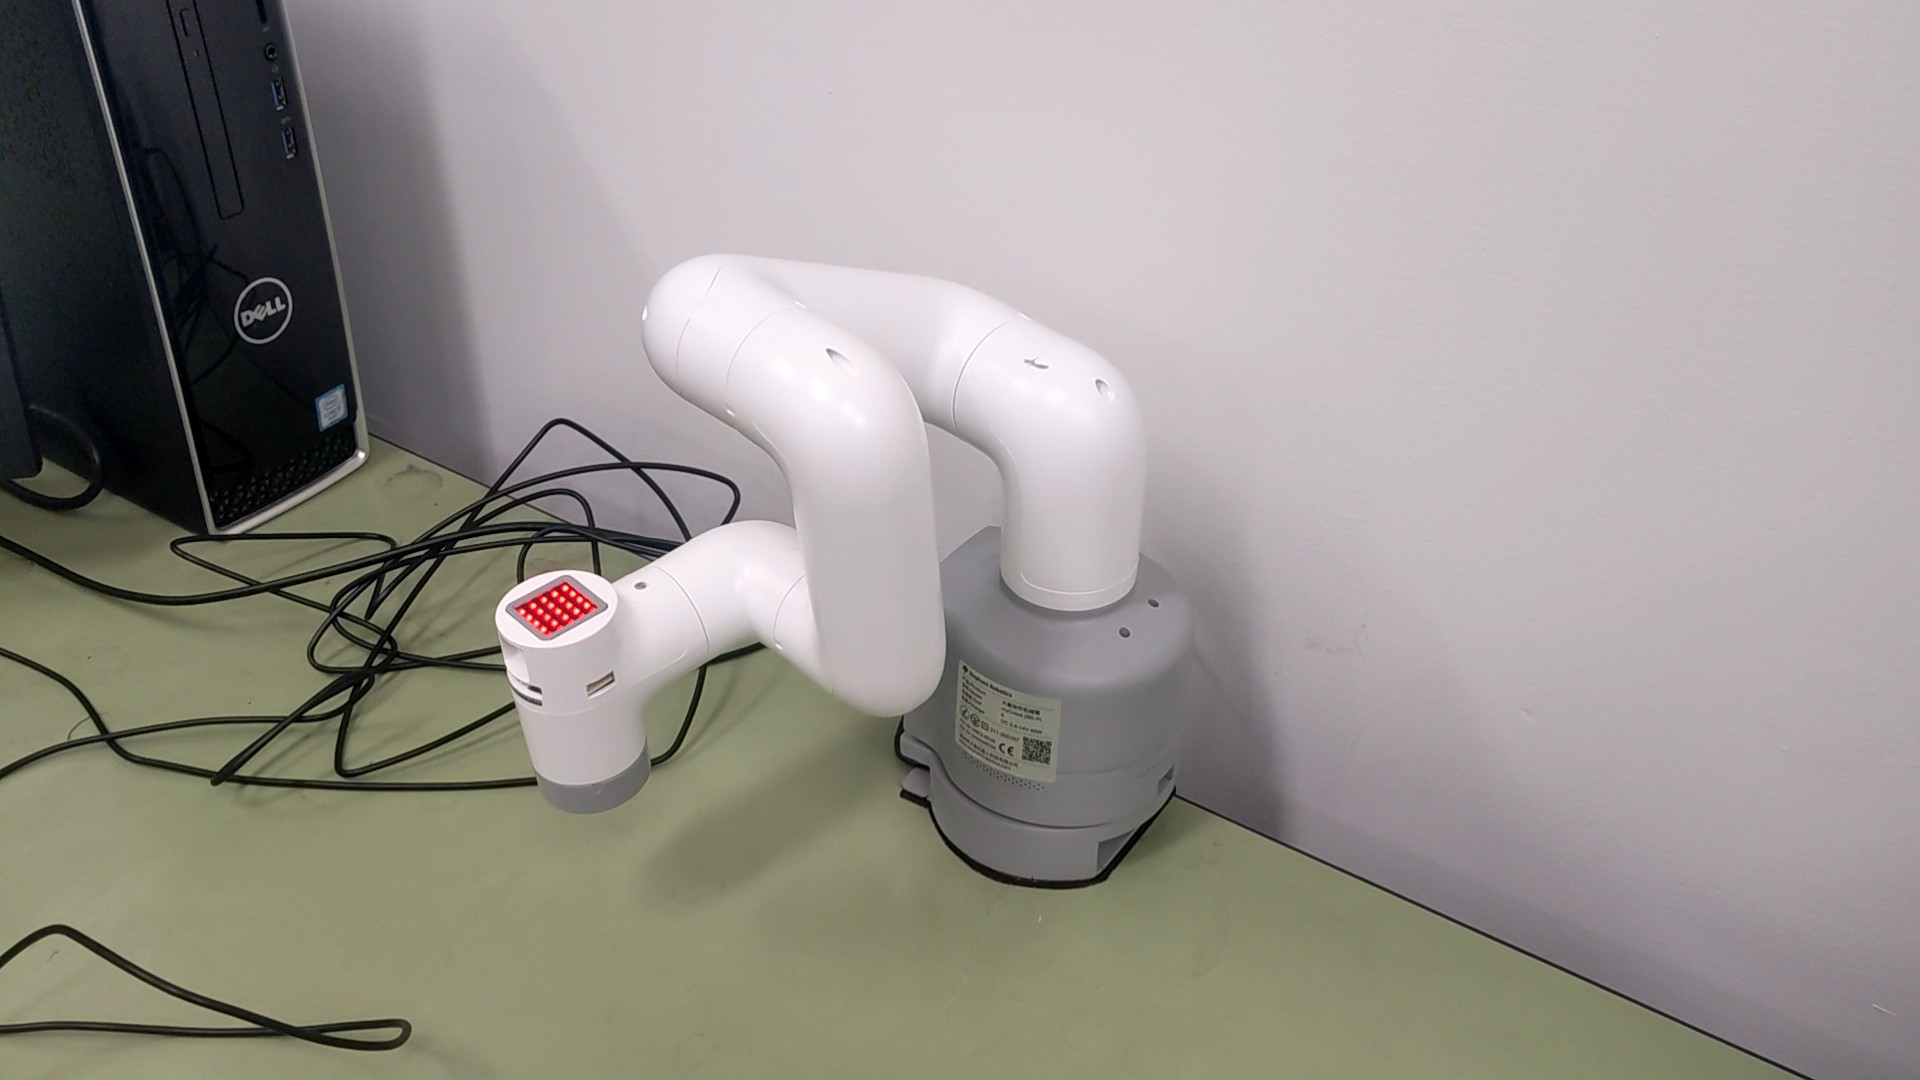
\includegraphics[width = 0.96\linewidth]{../results/program10_1.jpg}
			\subcaption{初期位置$\mqty[150 & -100 & 50 & 1]^\mathsf{T}$}
		\end{minipage}
		&
		\begin{minipage}[c]{0.48\linewidth}
			\centering
			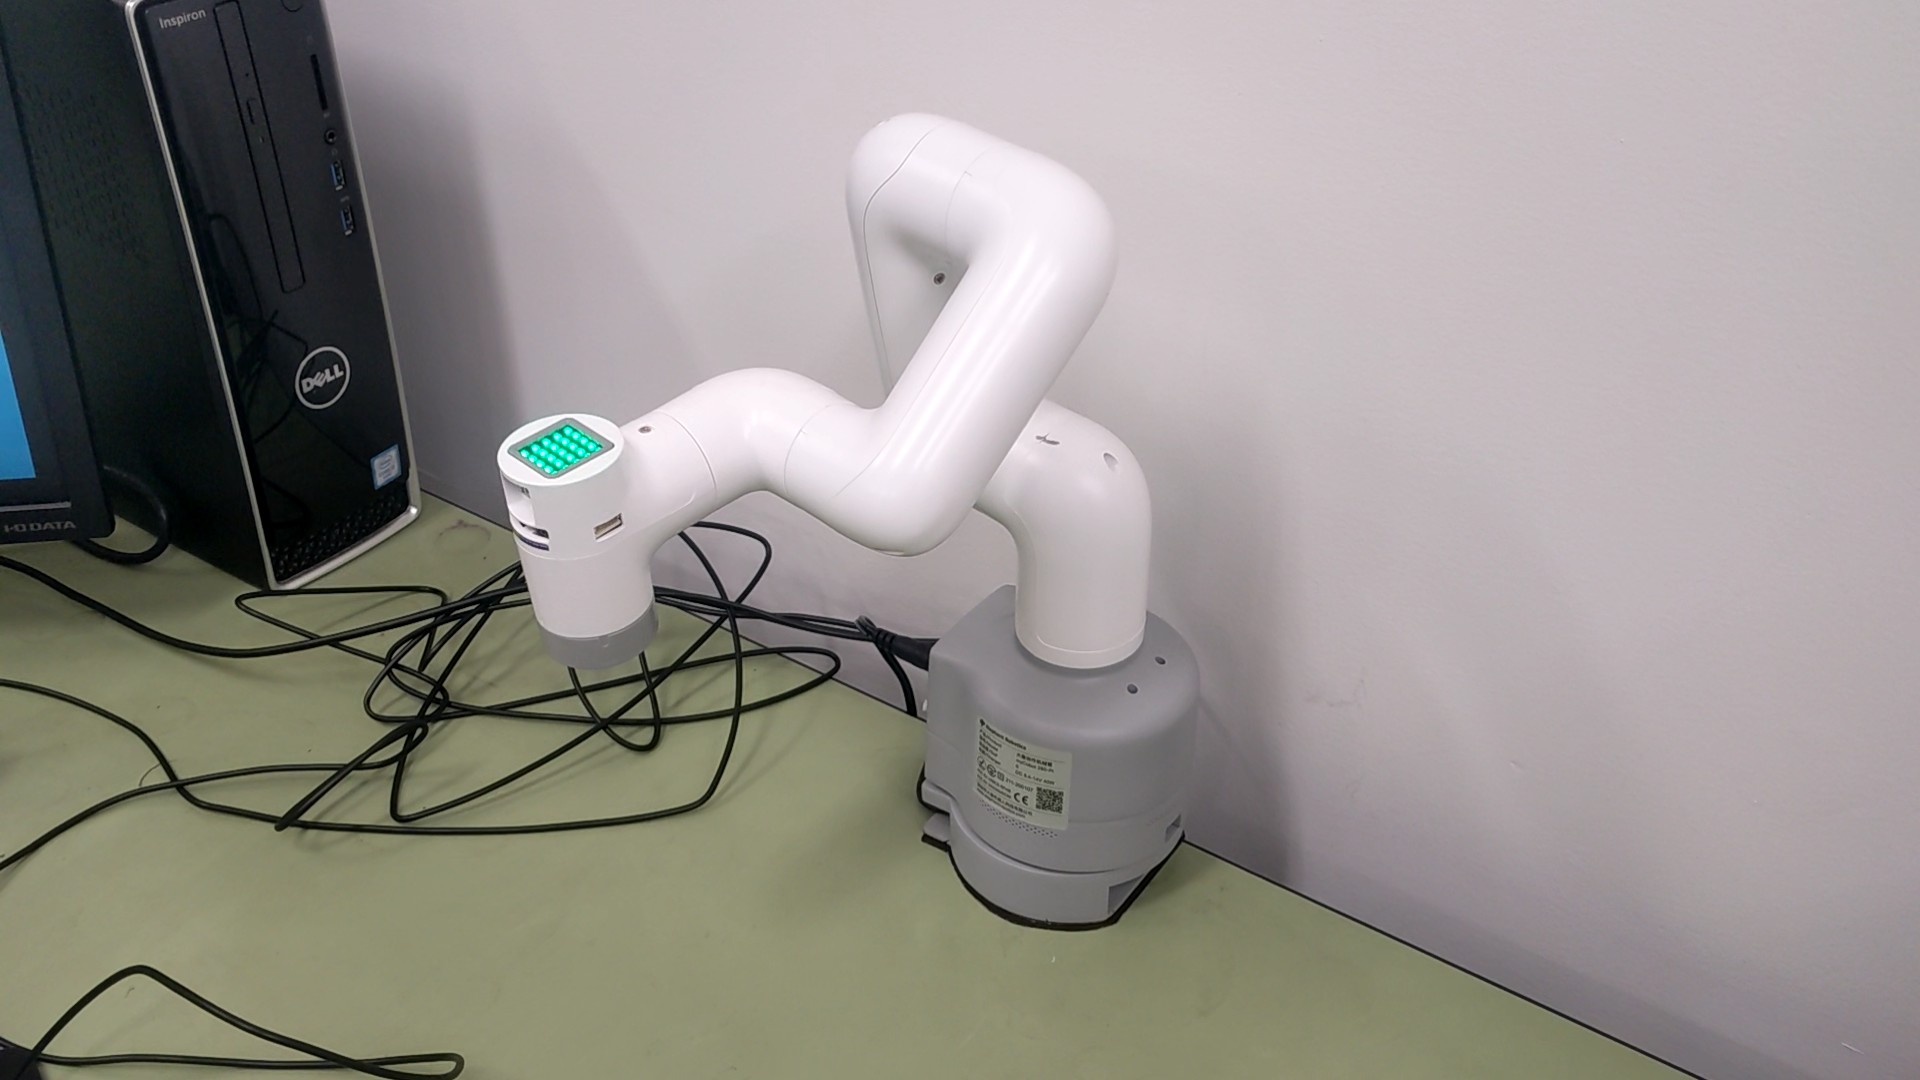
\includegraphics[width = 0.96\linewidth]{../results/program10_2.jpg}
			\subcaption{初期位置上空$\mqty[150 & -100 & 150 & 1]^\mathsf{T}$}
		\end{minipage}
		\\
		\begin{minipage}[c]{0.48\linewidth}
			\centering
			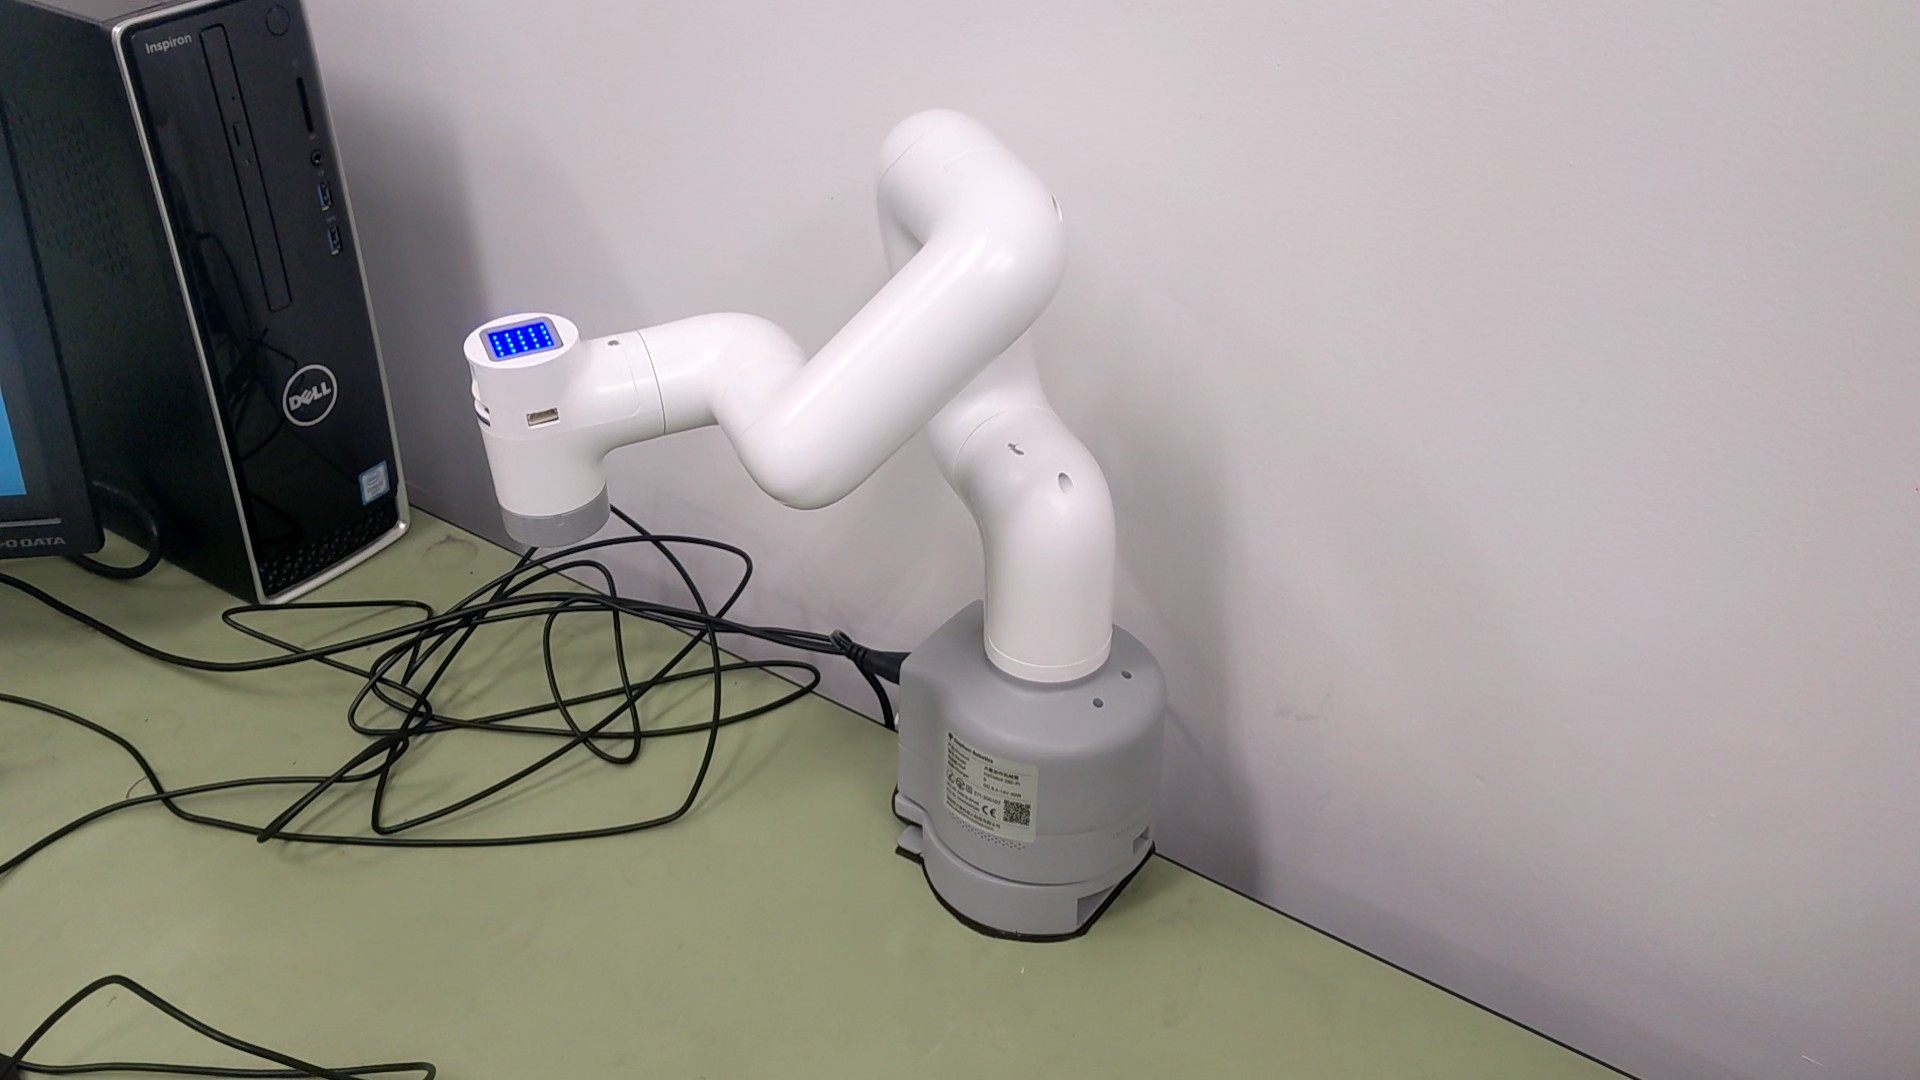
\includegraphics[width = 0.96\linewidth]{../results/program10_3.jpg}
			\subcaption{最終位置上空$\mqty[100 & -150 & 150 & 1]^\mathsf{T}$}
		\end{minipage}
		&
		\begin{minipage}[c]{0.48\linewidth}
			\centering
			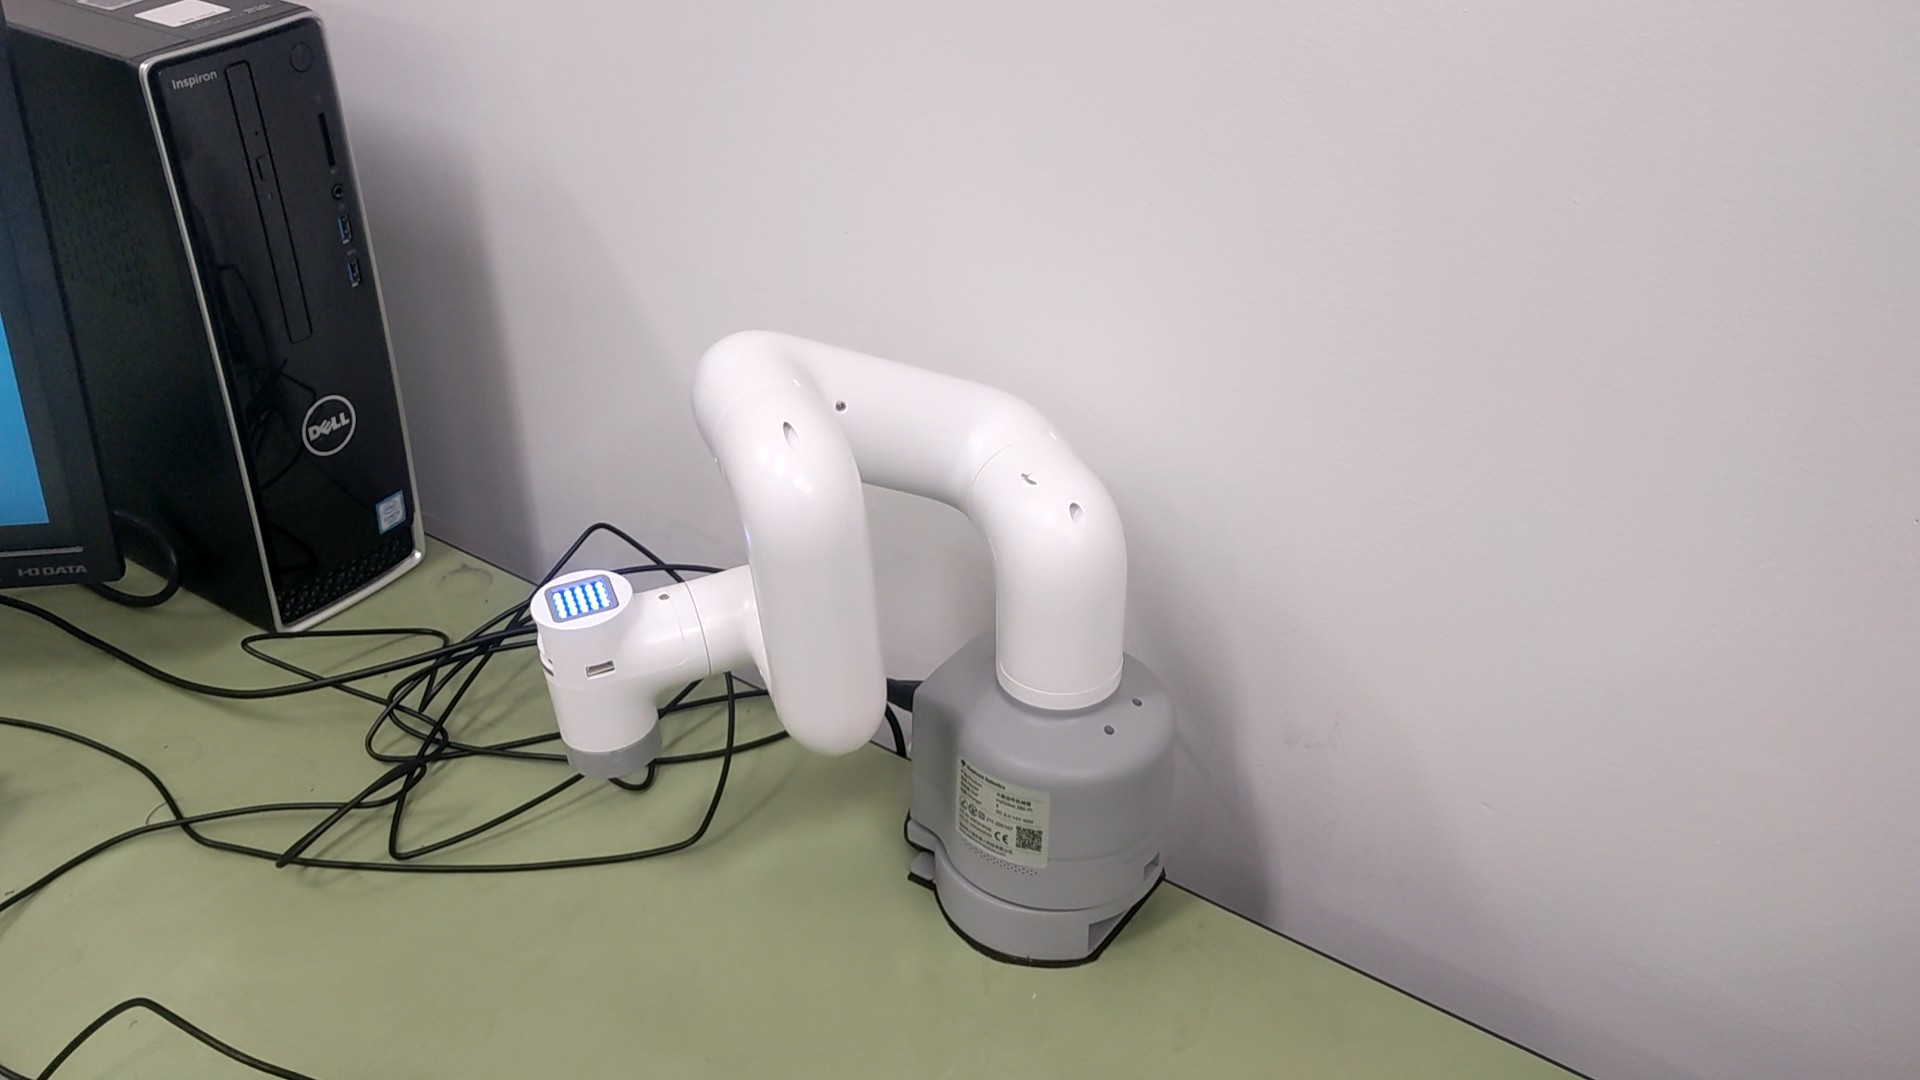
\includegraphics[width = 0.96\linewidth]{../results/program10_4.jpg}
			\subcaption{最終位置$\mqty[100 & -150 & 50 & 1]^\mathsf{T}$}
		\end{minipage}
	\end{tabular}
	\caption{初期位置から最終位置までの運搬のようす(実機)}
	\label{fig:初期位置から最終位置までの運搬のようす-実機}
\end{figure}

\printbibliography[title=参考文献]

\section*{付録}
\lstinputlisting[caption=同次変換行列の積を計算するプログラム,label=src:同次変換行列の積を計算するプログラム]{../src/calc_forward_kinematics.py}
\lstinputlisting[caption=6関節角度を入力し,全関節を同時に動作させるプログラム,label=src:6関節角度を入力し,全関節を同時に動作させるプログラム]{../src/program2.py}
\lstinputlisting[caption=順運動学により,関節角度から手先位置を計算するプログラムの作成,label=src:順運動学により,関節角度から手先位置を計算するプログラムの作成]{../src/program3.py}
\lstinputlisting[caption=$Z$方向の手先位置が\SI{15}{\mm}以内の場合にエラーを発生させるプログラム,label=src:Z方向の手先位置が15mm以内の場合にエラーを発生させるプログラム]{../src/program4.py}
\lstinputlisting[caption=逆運動学により入力した位置に手先を移動させるプログラム,label=src:逆運動学により入力した位置に手先を移動させるプログラム]{../src/program7.py}
\lstinputlisting[caption=初期位置にあるプレートを最終位置に移動させるプログラム,label=src:初期位置にあるプレートを最終位置に移動させるプログラム]{../src/program8.py}
\lstinputlisting[caption=初期位置にあるプレートを最終位置に移動させるプログラム(実機),label=src:初期位置にあるプレートを最終位置に移動させるプログラム-実機]{../src/program10.py}

\end{document}